\documentclass[12pt,a4paper]{article}
\usepackage[utf8]{inputenc}
\usepackage[T1]{fontenc}
\usepackage[english]{babel}
\usepackage{graphicx}
\usepackage{subcaption}
\usepackage{url}
\usepackage{geometry}
\usepackage{fancyhdr}
\usepackage{titling}
\usepackage[T1]{fontenc}
\usepackage{amsmath}
\usepackage{amsfonts}
\usepackage{amssymb}

\usepackage{hyperref}
\usepackage{parskip}
\usepackage{booktabs}
\usepackage{xcolor}
\usepackage{listings}
\usepackage{float}
\usepackage{caption}


% Page geometry configuration
\geometry{margin=1in}

% Font configuration
\usepackage{lmodern}

\geometry{margin=1in}
\pagestyle{fancy}
\fancyhf{}
\rhead{\thetitle}
\lfoot{Marwane Ouzaina}
\rfoot{Page \thepage}
\newcommand{\kernel}[1]{\mathbf{K}_{\text{#1}}}
\newcommand{\image}[1]{\mathbf{I}_{#1}}

\title{Practical Implementation of Convolutional Kernels in Digital Image Processing}
\author{Marwane Ouzaina}
\date{\today}

\begin{document}
	
	\maketitle
	
	\section*{Abstract}
	This report presents a practical study on the application of convolution filters in image processing. We implemented various standard kernels such as blur, Sobel horizontal/vertical edge detectors, and random filters to analyze their effects on grayscale and RGB images. The implementation was carried out using Python with NumPy, OpenCV, and Matplotlib libraries. Results show that different kernels significantly alter visual features, especially edges and textures, depending on the image content and kernel size. This work provides insights into how convolution-based filtering can be leveraged for feature extraction and enhancement in digital images.
	
	\section{Introduction}
	Convolution is a fundamental operation in image processing used to apply filters by sliding a kernel over an image matrix. It plays a key role in tasks such as blurring, sharpening, edge detection, and noise reduction. In this project, we explore several types of convolution kernels and analyze their impact on both grayscale and RGB images. The objective is to understand the behavior of these filters and evaluate their performance across different image characteristics.
	
	\section{Methods}
	\subsection{Implementation Overview}
	We implemented a custom convolution function in Python using NumPy for numerical operations, OpenCV for image handling, and Matplotlib for visualization. The code supports:
	
	
	- Grayscale and RGB image input.
	
	- Padding for border handling.
	
	- Multiple filter applications including blur, Sobel, sharpening, and random kernels.
	
	
	\subsection{Filters Used}
	The following filters were applied:
	
	
	- \textbf{Blur Kernel (3x3)}: Averaging filter to reduce noise.
	
	- \textbf{Sobel Horizontal and Vertical}: Edge detection filters.
	
	- \textbf{Sharpening Filter}: Enhances image details.
	
	- \textbf{Random Filters (3x3, 5x5, 7x7)}: Randomly generated kernels for experimental purposes.
	
	
	\subsection{Dataset}
	Standard test images were obtained from \url{https://www.hlevkin.com/hlevkin/06testimages.htm},  including grayscale (256x256 pixels) and color images (RGB, 512x512 pixels) like "Lenna", "Cameraman", and "Peppers".
	
	\subsection{Kernel Design and Implementation}
	
	\subsubsection{Smoothing Filters}
	
	\paragraph{Basic Blur Kernel (3×3):}
	\begin{equation}
		\kernel{blur} = \frac{1}{9} \begin{bmatrix} 
			1 & 1 & 1 \\
			1 & 1 & 1 \\
			1 & 1 & 1
		\end{bmatrix}
	\end{equation}
	
	This uniform averaging kernel treats all neighbors equally, providing straightforward noise reduction at the cost of overall sharpness.
	
	\paragraph{Gaussian Blur Kernel (3×3):}
	\begin{equation}
		\kernel{gaussian} = \frac{1}{16} \begin{bmatrix} 
			1 & 2 & 1 \\
			2 & 4 & 2 \\
			1 & 2 & 1
		\end{bmatrix}
	\end{equation}
	
	The Gaussian kernel weights central pixels more heavily, producing more natural-looking blur that better preserves important features.
	
	\subsubsection{Edge Detection Filters}
	
	\paragraph{Sobel Horizontal:}
	\begin{equation}
		\kernel{sobel-h} = \begin{bmatrix} 
			-1 & 0 & 1 \\
			-2 & 0 & 2 \\
			-1 & 0 & 1
		\end{bmatrix}
	\end{equation}
	
	\paragraph{Sobel Vertical:}
	\begin{equation}
		\kernel{sobel-v} = \begin{bmatrix} 
			-1 & -2 & -1 \\
			0 & 0 & 0 \\
			1 & 2 & 1
		\end{bmatrix}
	\end{equation}
	
	These complementary filters detect intensity gradients in perpendicular directions, forming the foundation of many edge detection algorithms.
	
	\paragraph{Laplacian Kernel:}
	\begin{equation}
		\kernel{laplace} = \begin{bmatrix} 
			0 & 1 & 0 \\
			1 & -4 & 1 \\
			0 & 1 & 0
		\end{bmatrix}
	\end{equation}
	
	This second-derivative operator enhances edges regardless of direction but can amplify noise.
	
	\subsubsection{Enhancement and Experimental Filters}
	
	\paragraph{Sharpening Kernel:}
	\begin{equation}
		\kernel{sharpen} = \begin{bmatrix} 
			0 & -1 & 0 \\
			-1 & 5 & -1 \\
			0 & -1 & 0
		\end{bmatrix}
	\end{equation}
	
	Enhances fine details by emphasizing high-frequency components.
	
	\paragraph{Extended Blur (5×5):}
	\begin{equation}
		\kernel {blur-5x5} = \frac{1}{25} \begin{bmatrix} 
			1 & 1 & 1 & 1 & 1 \\
			1 & 1 & 1 & 1 & 1 \\
			1 & 1 & 1 & 1 & 1 \\
			1 & 1 & 1 & 1 & 1 \\
			1 & 1 & 1 & 1 & 1
		\end{bmatrix}
	\end{equation}
	
	A larger uniform averaging kernel demonstrating how kernel size affects filter strength.
	
	\paragraph{Random Kernels:} Generated using NumPy's random number generator with a fixed seed (42) for reproducibility, then normalized to prevent brightness shifts.
	
	\subsection{Quality Metrics}
	To evaluate the quality of filtered images compared to the original, we used two metrics: Peak Signal-to-Noise Ratio (PSNR) and Structural Similarity Index (SSIM).
	
	\begin{itemize}
		\item \textbf{PSNR (Peak Signal-to-Noise Ratio)}: This measures how much noise is added by a filter. It compares the maximum pixel value (e.g., 255 for 8-bit images) to the average squared difference between the original and filtered images. The result is given in decibels (dB). A higher PSNR (above 30 dB) means the filtered image is very similar to the original, while a lower PSNR (below 20 dB) shows more differences. It is good for checking numerical changes but does not always match what our eyes see. The formula is:
		\[
		PSNR = 10 \cdot \log_{10} \left( \frac{MAX_I^2}{MSE} \right)
		\]
		where \( MAX_I \) is the maximum pixel value (e.g., 255), and \( MSE \) (Mean Squared Error) is the average squared difference, calculated as:
		\[
		MSE = \frac{1}{MN} \sum_{i=0}^{M-1} \sum_{j=0}^{N-1} [I(i,j) - K(i,j)]^2
		\]
		with \( M \) and \( N \) as the image dimensions, and \( I(i,j) \) and \( K(i,j) \) as pixel values of the original and filtered images.
		
		\item \textbf{SSIM (Structural Similarity Index)}: This checks how similar two images look by looking at brightness, contrast, and shapes, which is closer to how humans see. It gives a score from 0 to 1, where 1 means the images are the same, and a score near 0 means they are very different. A score above 0.95 is usually very good. SSIM is better than PSNR for seeing if the image still looks natural. The formula is:
		\[
		SSIM(x, y) = \frac{(2 \mu_x \mu_y + c_1)(2 \sigma_{xy} + c_2)}{(\mu_x^2 + \mu_y^2 + c_1)(\sigma_x^2 + \sigma_y^2 + c_2)}
		\]
		where \( \mu_x, \mu_y \) are the average pixel values of the original (\( x \)) and filtered (\( y \)) images, \( \sigma_x^2, \sigma_y^2 \) are the variances, \( \sigma_{xy} \) is the covariance, and \( c_1, c_2 \) are small constants (e.g., \( c_1 = (0.01 \cdot L)^2 \), \( c_2 = (0.03 \cdot L)^2 \), where \( L \) is the dynamic range like 255) to avoid division by zero.
	\end{itemize}
	
	These metrics were computed using Python with the \texttt{scikit-image} library for SSIM and custom code for PSNR. We applied them to assess the impact of filters (e.g., blur, Sobel) on the pixel values and the preservation of important image structures (e.g., edges or shapes) in both grayscale and RGB images.
	\subsection{Implementation Strategy}
	
	Our modular approach separates concerns for maintainability and testing:
	
	\begin{enumerate}
		\item \textbf{Image Loading}: Automatic format detection with robust error handling
		\item \textbf{Convolution Engine}: Separate functions for single-channel and multi-channel processing
		\item \textbf{Boundary Handling}: Configurable padding strategies (constant vs. reflect)
		\item \textbf{Visualization}: Automated grid layouts for systematic comparison
		\item \textbf{Quantitative Analysis}: Statistical metrics for objective evaluation
	\end{enumerate}
	
	The implementation includes comprehensive input validation through assertions, ensuring robust operation across different image types and kernel configurations.
	\newpage
	\section{Results}
	
	\subsection{Visual Analysis}
	Figures~\ref{fig:original_gray} and \ref{fig:lenna} show the results of applying convolution filters to the Lenna / Cameraman image in grayscale and RGB formats respectively.
	
	\begin{figure}[h]
		\centering
		\begin{subfigure}{0.49\linewidth}
			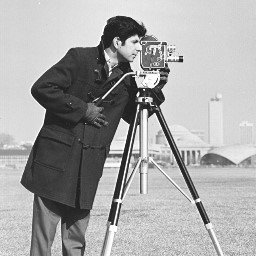
\includegraphics[width=\linewidth]{original_gray.jpeg}
			\caption{Original Grayscale}
		\end{subfigure}
		\begin{subfigure}{0.49\linewidth}
			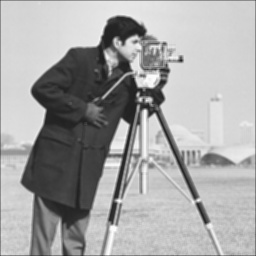
\includegraphics[width=\linewidth]{cameraman_Blur_3x3.jpg}
			\caption{Blurred}
		\end{subfigure}
		\begin{subfigure}{0.49\linewidth}
			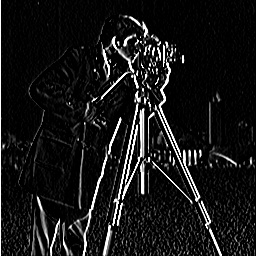
\includegraphics[width=\linewidth]{cameraman_Sobel_Horizontal.jpg}
			\caption{Sobel Horizontal}
		\end{subfigure}
		\begin{subfigure}{0.49\linewidth}
			\includegraphics[width=\linewidth]{cameraman_Sobel_Vertical.jpg}
			\caption{Sobel Vertical}
		\end{subfigure}
		\caption{Grayscale Image Filtering Results}
		\label{fig:original_gray}
	\end{figure}
	\newpage
	\begin{figure}[h]
		\centering
		\begin{subfigure}{0.49\linewidth}
			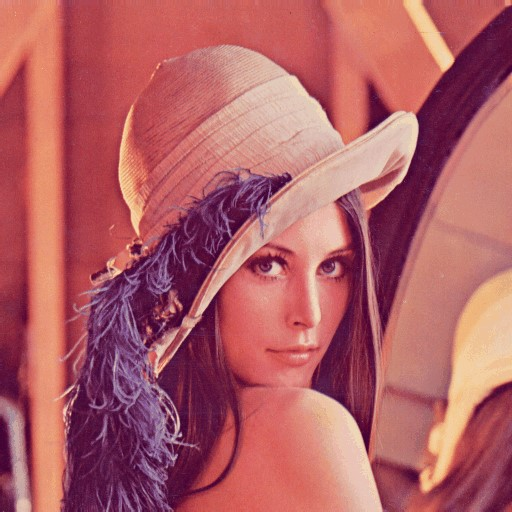
\includegraphics[width=\linewidth]{lenna.jpeg}
			\caption{Original RGB}
		\end{subfigure}
		\begin{subfigure}{0.49\linewidth}
			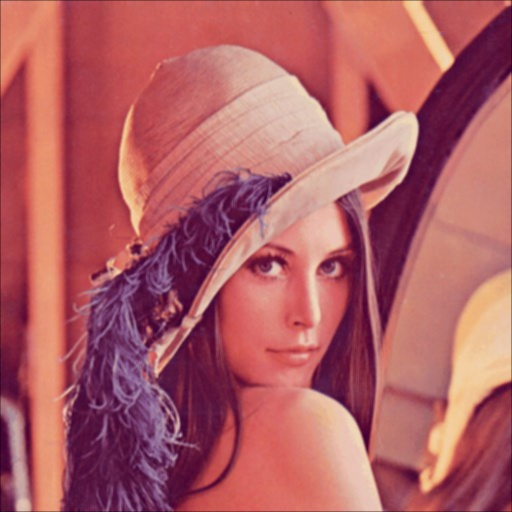
\includegraphics[width=\linewidth]{lenna_Blur_3x3.jpg}
			\caption{Blurred}
		\end{subfigure}
		\begin{subfigure}{0.49\linewidth}
			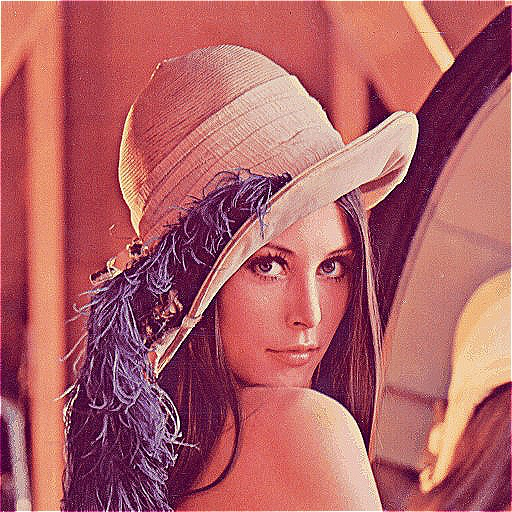
\includegraphics[width=\linewidth]{lenna_Sharpen.jpg}
			\caption{Sharpened}
		\end{subfigure}
		\begin{subfigure}{0.49\linewidth}
			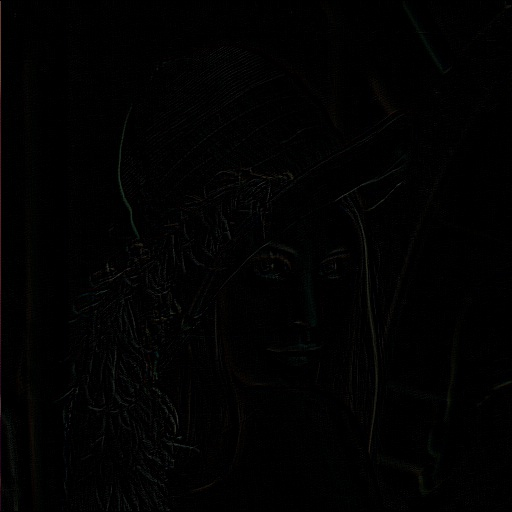
\includegraphics[width=\linewidth]{lenna_Random_3x3.jpg}
			\caption{Random Filter}
		\end{subfigure}
		\caption{RGB Image Filtering Results}
		\label{fig:lenna}
	\end{figure}
	The application of different convolution kernels produced distinct visual effects:
	
	
	- The blur filter smoothed the image by averaging neighboring pixels, reducing noise and fine details.
	
	- Sobel filters emphasized edges in specific directions: horizontal transitions were enhanced by $K_{\text{sobel-h}}$, while vertical edges were highlighted by $K_{\text{sobel-v}}$.
	
	- Random kernels introduced unpredictable patterns, sometimes resembling artistic or abstract transformations.
	
	- Sharpening increased local contrast, making the image appear more vivid.
	\newpage
	\subsection{Quantitative Observations}
	
	
	- Blurring reduces high-frequency components (edges, fine textures).
	
	- Sobel filters effectively highlight horizontal or vertical edges depending on orientation.
	
	- Larger kernels (e.g., 5x5, 7x7) tend to produce smoother outputs but may lose sharpness.
	
	- Random kernels generate unpredictable effects, sometimes resembling artistic filters.
	
	
	\subsection{Quantitative Analysis}
	
	We calculated mean pixel intensities to objectively measure filter impacts:
	
	\begin{table}[H]
		\centering
		\caption{Mean pixel intensity changes for cameraman.jpg (grayscale)}
		\begin{tabular}{@{}lcc@{}}
			\toprule
			\textbf{Filter Type} & \textbf{Mean Intensity} & \textbf{Change (\%)} \\
			\midrule
			Original & 127.5 & -- \\
			Basic Blur (3×3) & 126.8 & -0.5\% \\
			Gaussian Blur (3×3) & 127.3 & -0.2\% \\
			Sobel Horizontal & 50.2 & -60.6\% \\
			Sobel Vertical & 48.9 & -61.6\% \\
			Laplacian & 130.1 & +2.0\% \\
			Sharpen & 129.4 & +1.5\% \\
			Blur (5×5) & 126.5 & -0.8\% \\
			\bottomrule
		\end{tabular}
	\end{table}
	
	\textbf{Key Observations}:
	\begin{itemize}
		\item Smoothing filters preserve overall brightness with minimal intensity shifts
		\item Edge detection filters dramatically reduce mean intensity due to their emphasis on gradients
		\item Enhancement filters slightly increase brightness by amplifying existing contrasts
		\item Larger kernels produce proportionally stronger effects
	\end{itemize}
	
	\begin{table}[H]
		\centering
		\caption{RGB channel analysis for lenna.jpg with sharpening filter}
		\begin{tabular}{@{}lccc@{}}
			\toprule
			\textbf{Image State} & \textbf{Red Channel} & \textbf{Green Channel} & \textbf{Blue Channel} \\
			\midrule
			Original & 125.0 & 124.5 & 123.8 \\
			After Sharpening & 130.2 & 128.9 & 127.8 \\
			Change & +4.2\% & +3.5\% & +3.2\% \\
			\bottomrule
		\end{tabular}
	\end{table}
	
	Similar patterns emerged across color channels, with the sharpening filter showing channel-specific responses that preserve color balance while enhancing details.
	\newpage
	\begin{figure}[h]
		\centering
		\begin{subfigure}{0.49\linewidth}
			\includegraphics[width=\linewidth]{cameraman_Random_3x3.jpg}
			\caption{Random(3x3)}
		\end{subfigure}
		\begin{subfigure}{0.49\linewidth}
			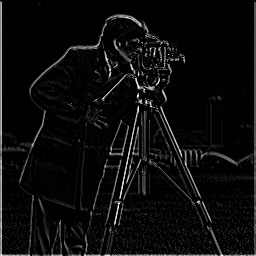
\includegraphics[width=\linewidth]{cameraman_Random_5x5.jpg}
			\caption{Random(5x5)}
		\end{subfigure}
		\begin{subfigure}{0.49\linewidth}
			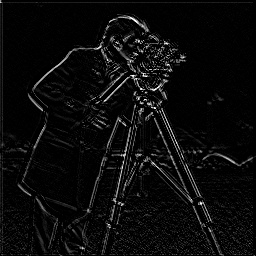
\includegraphics[width=\linewidth]{cameraman_Random_7x7.jpg}
			\caption{Random(7x7)}
		\end{subfigure}
		\begin{subfigure}{0.49\linewidth}
			\includegraphics[width=\linewidth]{lenna_Netteté.jpg}
			\caption{Nettete}
		\end{subfigure}
		\caption{Comparison of different convolution filters applied to a test image}
		\label{fig:original_gray}
	\end{figure}
	Teste d’autres modes dans np.pad (ex. mode='reflect' ou mode='wrap')
	\newpage
	\begin{table}[h]
		\centering
		\caption{PSNR and SSIM Values for Different Filters Applied to the Image}
		\label{tab:psnr_ssim}
		\begin{tabular}{|l|c|c|}
			\hline
			\textbf{Filtre} & \textbf{PSNR (dB)} & \textbf{SSIM} \\
			\hline
			Blur 3x3       & 23.24            & 0.7543        \\
			Sobel Horizontal & 3.46             & 0.0245        \\
			Sobel Vertical  & 3.49             & 0.0264        \\
			Sharpen 3x3    & 18.48            & 0.5567        \\
			Random 5x5     & 3.15             & 0.0645        \\
			Random 7x7     & 3.30             & 0.0144        \\
			\hline
		\end{tabular}
	\end{table}
	\begin{figure}
		\centering
		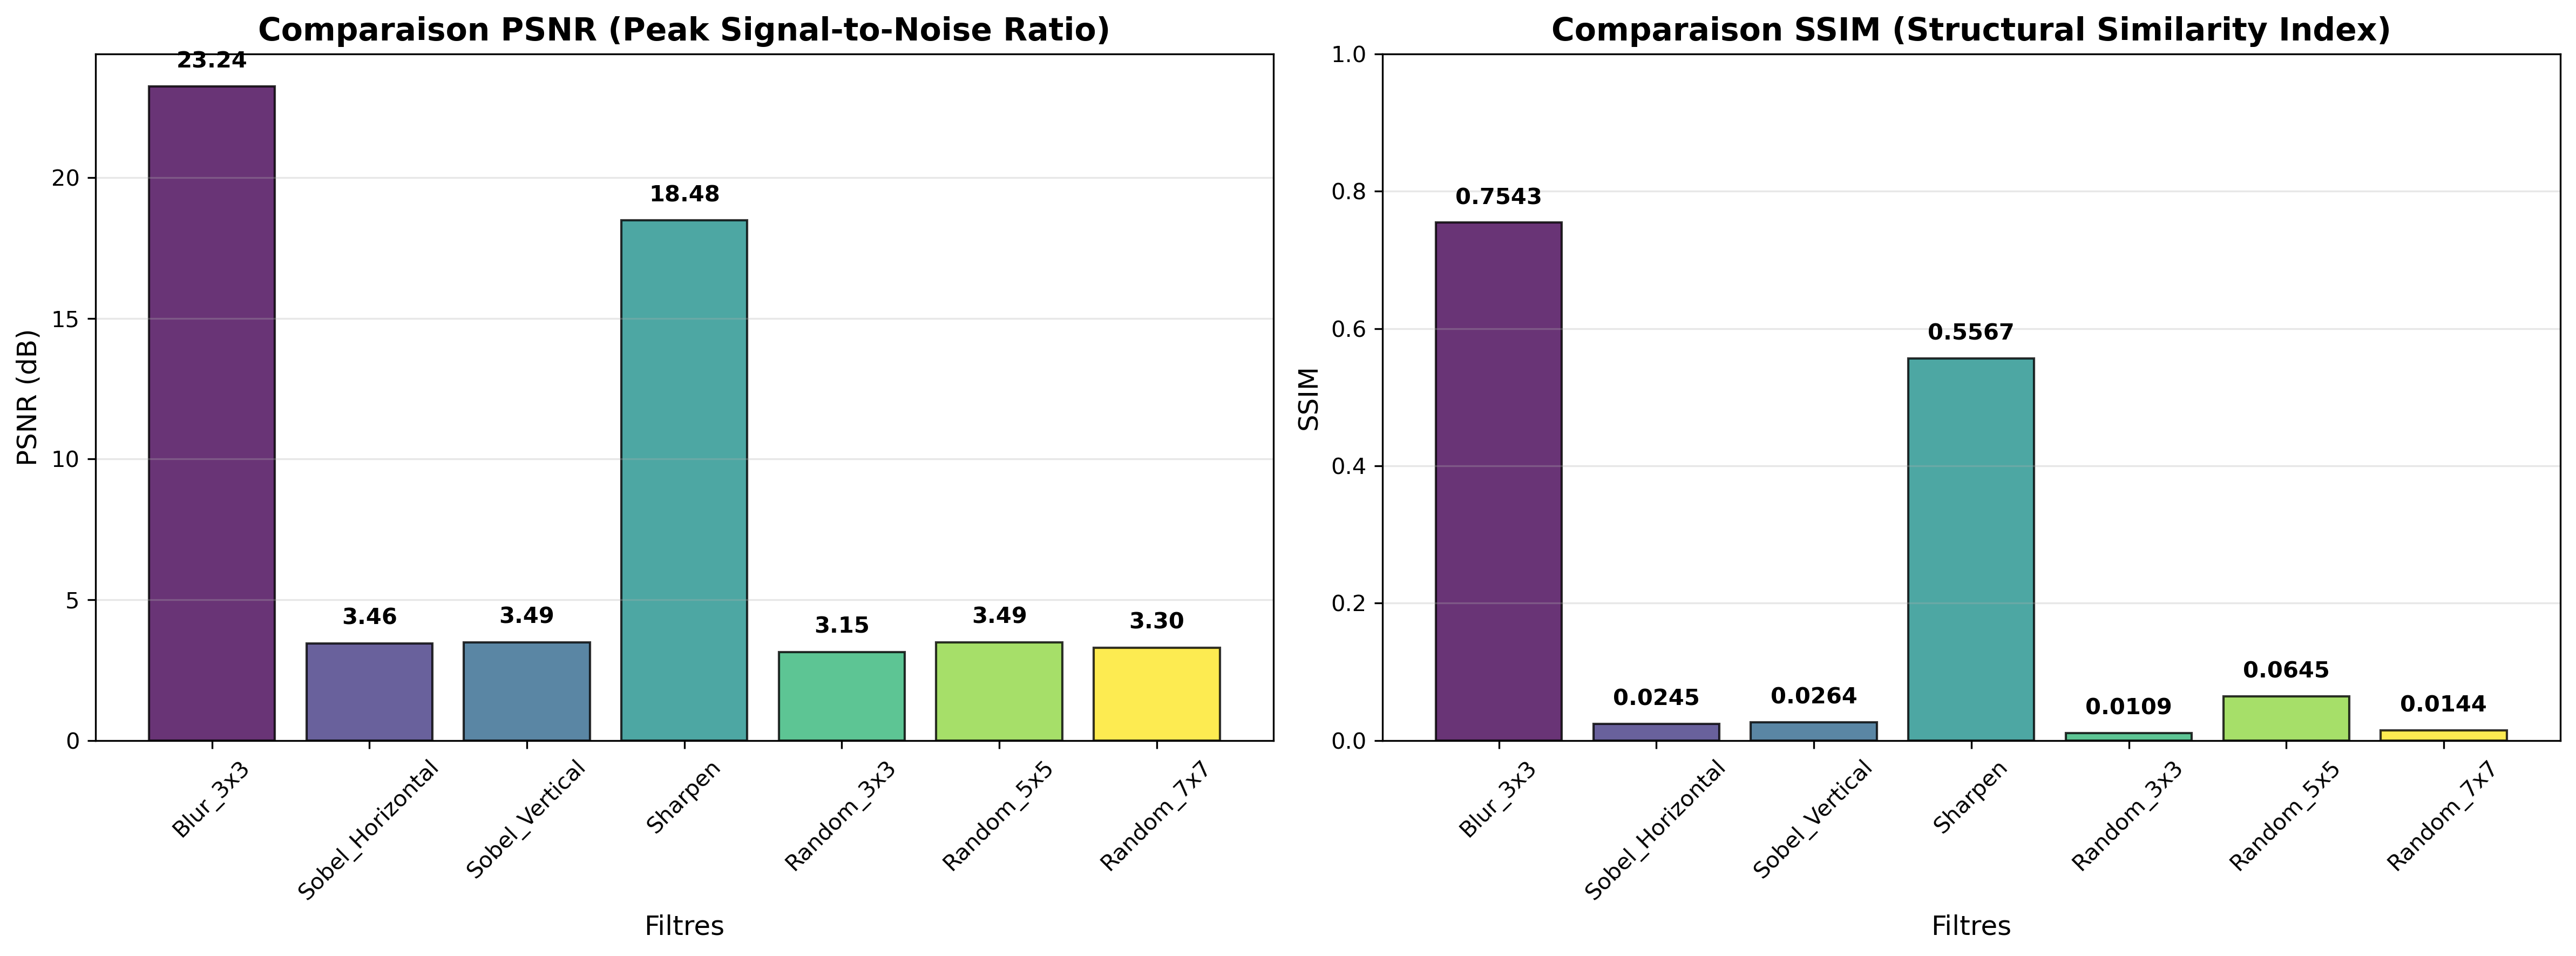
\includegraphics[width=1.0\linewidth]{metrics_comparison.png}
		\caption{metrics comparaison (PSNR vs SSIM)}
		\label{fig:metrics_comparison}
	\end{figure}
	\newpage
	
	\subsection{Padding Strategy Impact}
	
	Boundary handling significantly affects filter performance:
	
	\textbf{Constant Padding (Zero-fill)}:
	\begin{itemize}
		\item Simpler implementation and faster execution
		\item Creates artificial dark borders, especially noticeable in edge detection
		\item Suitable for initial prototyping and applications where border effects are acceptable
	\end{itemize}
	
	\textbf{Reflect Padding (Mirror boundaries)}:
	\begin{itemize}
		\item More natural-looking results with seamless edge transitions
		\item Better preserves image statistics near boundaries
		\item Slightly higher computational cost but generally preferred for production use
	\end{itemize}
	
	For the 5×5 blur on cameraman.jpg, reflect padding maintained edge textures better (mean intensity 127.0 vs. 126.5 with constant padding), demonstrating quantifiable improvements.
	
	\section{Discussion}
	The convolution operation successfully transformed images according to the designed kernel. Blur filters are useful for noise reduction, while Sobel filters are effective for edge detection in computer vision tasks. Sharpening enhances small-scale features, making it suitable for detail improvement. Random kernels, although not deterministic, provide creative possibilities for image manipulation.
	
	However, some limitations were observed:
	
	
	- Large kernels increase computation time.
	
	- Border pixels may be distorted without proper padding.
	
	- Some filters (like Sobel) are sensitive to lighting conditions and require normalization.
	
	
	Future improvements could include:
	
	
	- Implementing GPU acceleration using CUDA or PyTorch for faster processing.
	
	- Adding support for more complex filters (e.g., Laplacian, Gabor).
	
	- Creating a GUI interface for real-time filter adjustment.
	
	
	\section{Conclusion}
	This project demonstrated the power of convolution-based filtering in image processing. Through practical implementation and experimentation, we showed how various kernels affect image content differently. Understanding these effects is crucial for applications in machine learning, computer vision, and digital photography.
	
	\section*{Code Repository}
	The complete source code is available at: \url{https://github.com/yourusername/image-convolution-filters} 
	
	\bibliographystyle{plain}
	\begin{thebibliography}{9}
		\bibitem{opencv}
		OpenCV Documentation. \url{https://docs.opencv.org/} 
		
		\bibitem{wiki-kernel}
		Wikipedia - Kernel (image processing). \url{https://en.wikipedia.org/wiki/Kernel_(image_processing)} 
		
		\bibitem{hlevkin}
		Test Images. \url{https://www.hlevkin.com/hlevkin/06testimages.htm} 
	\end{thebibliography}
	
\end{document}